\chapter{NEORV32's space address} \label{chp:chapter_s}

    \begin{figure}[!ht]
        \begin{center}
            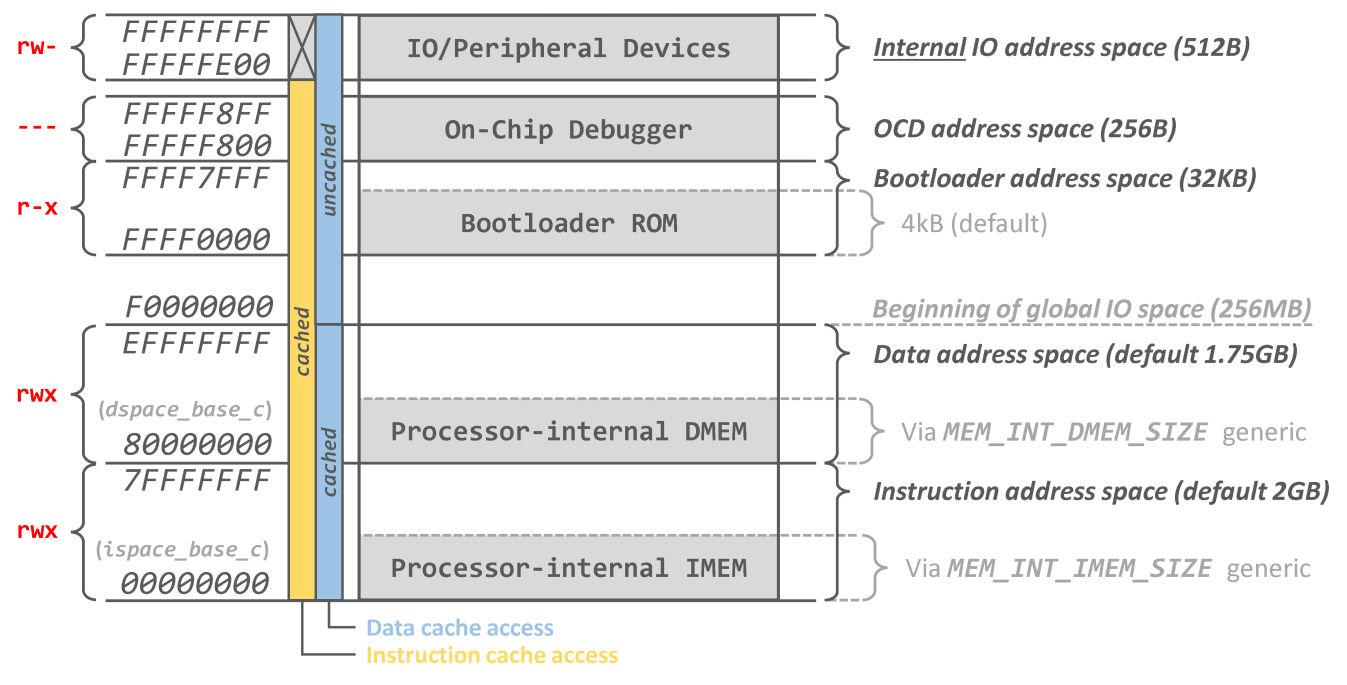
\includegraphics[width=\textwidth]{figures/address_space.png}
            \caption{\label{fig:neorv32_address_space} Representation of the NEORV32's space address.}
        \end{center}
    \end{figure}

    Welcome to the \autoref{chp:chapter_s}. Here we are going to present the NEORV32's memory regions. The NEORV32 is a 32-bit architecture, which have access to up to 4GB memory. By default, this address space is divided into five main regions, as presented in \autoref{fig:neorv32_address_space}.

    \textbf{Instruction address space}: where the code itself and constants are going to be stored. This address space can be referenced as instruction memory (IMEM), and can go from 0x00000000 up to 0x7FFFFFFF.

        \begin{tcolorbox}[colback=blue!5!white,colframe=blue!75!black,title=Extra information]
            The implementation of the processor-internal data memory is enabled via the processor's MEM\_INT\_IMEM\_EN, a generic presented in \textit{neor32\_top.vhd} file. The size in bytes is defined via the MEM\_INT\_IMEM\_SIZE, which is by default 16x1024 bytes.
        \end{tcolorbox}

    \textbf{Data address space}: where the application run-time data (heap, stack, etc.) is stored. This address space can be referenced as data memory (DMEM), and can go from 0x80000000 up to 0xEFFFFFFF.

        \begin{tcolorbox}[colback=blue!5!white,colframe=blue!75!black,title=Extra information]
            The implementation of the processor-internal data memory is enabled via the processor's MEM\_INT\_DMEM\_EN, a generic presented in \textit{neor32\_top.vhd} file. The size in bytes is defined via the MEM\_INT\_DMEM\_SIZE, which is by default 8x1024 bytes.
        \end{tcolorbox}

    \textbf{Bootloader address space}: used for storing an optional built-in firmware that allows to upload new applications into the NEORV32. A UART connection is used to provide a simple text-based user interface that allows to upload the executable. This address space can be referenced as bootloader memory (BOOTROM), and can go from 0xFFFF0000 up to 0xFFFF7FFF.

    \textbf{IO/peripheral address space}: where the processor-internal memory-mapped peripherals are stored. Hence, all peripheral/IO devices are accessed using a memory-mapped scheme. It goes from 0xFFFFFE00 to 0xFFFFFFFF.


\chapter{NEORV32's peripherals}\label{chp:chapter_p}
 
    Welcome to the \autoref{chp:chapter_p}. Here we are going to show the theory behind the main NEORV32's peripherals that should be adapted to be used during the \textit{EEL7030 - Microprocessadores}. As presented in \autoref{fig:neorv32_peripherals}, some of the available peripherals are: UART, SPI, GPIO, PWM, TWI, interrupt controller, embedded memory and timers. Nevertheless, the UART, GPIO, interrupt controller and timers are the implemented ones, as are needed during the \textit{EEL7030}.

    \autoref{sec:section_p.1}: First, we are going to present the GPIO, a peripheral used to interface LEDs, 7-segments displays and LCD of the DE2i-150, as well as switches and buttons. We are going to present this peripheral and its implementation in the development board, showing the defined pin mapping. 
    
    \autoref{sec:section_p.2}: Then, the interrupt controller is presented. It is important to explain the concept of interrupt, trap and exceptions, mechanisms used by CPUs and microprocessor to identify a specific event that requires breaking the on-going execution flow, redirecting it to a interrupt service routine (ISR). The available interrupt sources are going to be presented, showing how to use them in the development board. 
    
    \autoref{sec:section_p.3}: Next, we will introduce timers, which are closely related to the previous peripheral, since they are often used to generate interruptions. Their utilization in the DE2i-150 is presented, too. 
    
    \autoref{sec:section_p.4}: Finally, reaching the end of the covered topics in the \textit{EEL7030}, we have the serial communications. Then, we will present the UART, the serial communication generally used in the course. We are going to explain what is an asynchronous and synchronous communication, how it is handled in the NEORV32 and, finally, show how it was implemented in the development board.
    
    \section{General-purpose input/output (GPIO)}\label{sec:section_p.1}

        The GPIO is composed by a set of programmable input/output pins that are used to provide an interface between external devices and the microprocessor. It can be fairly represented as in \autoref{fig:gpio_representation}. As configured as an output pin, it is possible to set it to high or low level, which means, respectively, VDD (3,3V, 5V or other common value) and GND. In this configuration, we still can read the pin's state. However, when configured as an input pin, it is no longer possible to set the pin's state, only being possible to read its state. The state that the pin should be set to, as well as its current state, is stored in registers, as can be seen in \autoref{fig:gpio_representation}.

        \begin{figure}[!ht]
            \begin{center}
                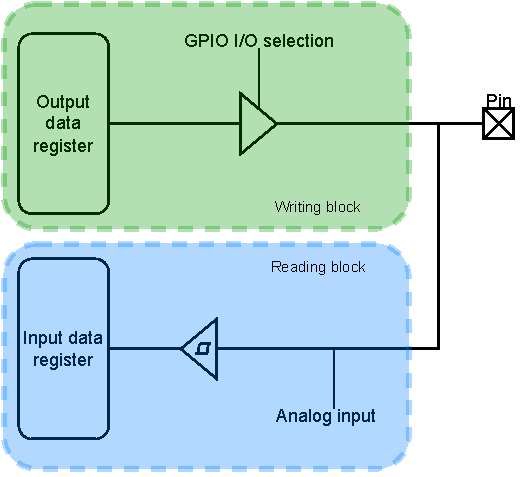
\includegraphics[width= 0.6\textwidth]{figures/gpio_representation.pdf}
                \caption{\label{fig:gpio_representation} Basic representation of a GPIO.}
            \end{center}
        \end{figure}

        \begin{table}[h]

        \centering
            \caption{\label{tab:register_map_gpio} GPIO's memory-mapped registers.}
            \begin{tabular}{ccccc}
                \toprule
                \textbf{Address} & \textbf{Name [C]} & \textbf{Bit(s)} & \textbf{R/W} & \textbf{Function} \\
                \midrule
                \midrule
                0xFFFFFFC0 & INPUT\_LO & 31:0 & r/- & parallel input port pins 31:0 \\ 
                0xFFFFFFC4 & INPUT\_HI & 31:0 & r/- & parallel input port pins 63:32 \\ 
                0xFFFFFFC8 & OUTPUT\_LO & 31:0 & r/w & parallel output port pins 31:0 \\ 
                0xFFFFFFCC & OUTPUT\_HI & 31:0 & r/w & parallel output port pins 63:32 \\ 
                \bottomrule
            \end{tabular}
        \end{table}

        The NEORV32 offers a simple parallel input and output port. These ports can be used chip-externally (for example to drive status LEDs, connect buttons, etc.) or chip-internally.

        \begin{tcolorbox}[colback=blue!5!white,colframe=blue!75!black,title=Extra information]
            The number of input/output pairs that will be available is defined by IO\_GPIO\_NUM, a generic presented in \textit{neor32\_top.vhd} file. When set to zero, the GPIO is excluded from synthesis and the output port is tied to all-zero. If IO\_GPIO\_NUM is less than the 64 (maximum value), only the LSB-aligned bits in gpio\_o and gpio\_i are actually connected while the remaining bits are tied to zero or are left unconnected, respectively.
        \end{tcolorbox}
        
        Furthermore, the GPIO's memory-mapped registers are presented in \autoref{tab:register_map_gpio}. To be able to control the pin's state, you should write to the address named OUTPUT\_HI (GPIO\_o [63:32]) and \textit{OUTPUT\_LO} (GPIO\_o [31:0]). Putting theses bits to ``1'' means that the pins are in high state, then putting them to ``0'' means that they are in low state. And to be able to see pin's states, you could read any of the 4 addresses. 

        Next, it will be presented the adaptation made to make it possible to use the NEORV32's GPIO in the DE2i-150. It will be also presented some theory behind LEDs, 7-segment displays and the LCDs.
        
        \subsection{LEDs}
            As we can see in \autoref{fig:led_fpga_board}, there are 27 user-controllable LEDs on the DE2i-150. Eighteen red LEDs and more 9 green LEDs. Nevertheless, only 8 red LEDs are available in the DE2i-150 (LEDR[8:0]), for general purposes. More 8 green LEDs are also available, to be used as status LEDs. \autoref{tab:ledg_o} and \autoref{tab:ledr_o} shows the assignments of the board's pins to the LEDs. 

            \begin{figure}[!ht]
                \begin{center}
                    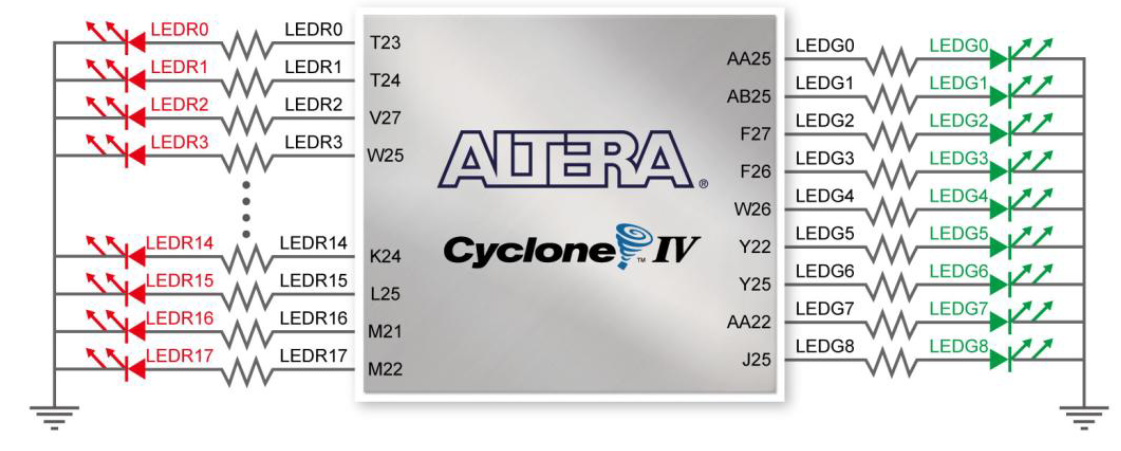
\includegraphics[width= 0.6\textwidth]{figures/led_fpga_board.png}
                    \caption{\label{fig:led_fpga_board} Available LEDs on the development board.}
                \end{center}
            \end{figure}
            
        \subsection{7-segment display}
           A 7-segment display is nothing more than a set of LEDs, positioned in such a way that they can form numbers and characters when correctly driven. The DE2i-150 has eight of these displays. Each segment is identified by an index, from 0 to 6, as presented in \autoref{figure:hex}. It is important to point out that each of these segments is going to be set to a high state when the pins connected to them are in low state. The \autoref{tab:hex} shows the assignments of the board's pins to the 7-segment displays.
            
                \begin{figure}[!ht]
                    \begin{center}
                        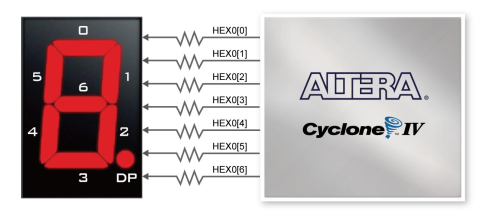
\includegraphics[width= 0.6\textwidth]{figures/chap2/hex.png}
                        \caption{\label{figure:hex} Connections between the 7-segment display HEX0 and Cyclone IV GX FPGA}
                    \end{center}
                \end{figure}
        
        \subsection{LCD}
            The DE2i-150 has a built-in LCD (the HD44780), too, and can be used to display text by sending appropriate commands to the display's controller. As presented in \autoref{figure:lcd}, there are some important signals to properly command de LCD: ON, DATA[7:0], EN, RS an RW. Basically, the LCD\_ON is used to power the LCD. The LCD\_DATA0 to LCD\_DATA7 are used to send a specific command (for instance, 38h, which is the command to define the interface and how many lines are going to be used) or to send a character in the display. Furthermore, LCD\_RW is used to define if we are going to read or write to the display and LCD\_RS is used to distinguish a read/write command from a read/write data to the LCD. Finally, the LCD\_EN is used to actually send the command and/or data whenever it is pulsed. The \autoref{tab:lcd_o} and \autoref{figure:lcd} shows the assignments of the board's pins to the LCD.
                
            \begin{figure}[!ht]
                \begin{center}
                    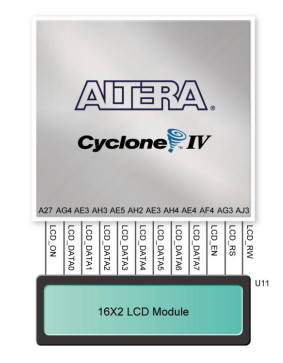
\includegraphics[width= 0.4\textwidth]{figures/chap2/lcd.png}
                    \caption{\label{figure:lcd} Connections between the LCD and Cyclone IV GX FPGA}
                \end{center}
            \end{figure}

        \subsection{Input/output pins}
            The DE2i-150 has 36 pins that can be used as input/output pins, as presented in \autoref{fig:pins_fpga_board}. But only 16 pins are going to be available to be used, where half are used as output pins and the other half as input pins. The \autoref{tab:gpio_o} and \autoref{tab:gpio_i} shows the assignments of the board's pins.
        
            \begin{figure}[!ht]
                \begin{center}
                    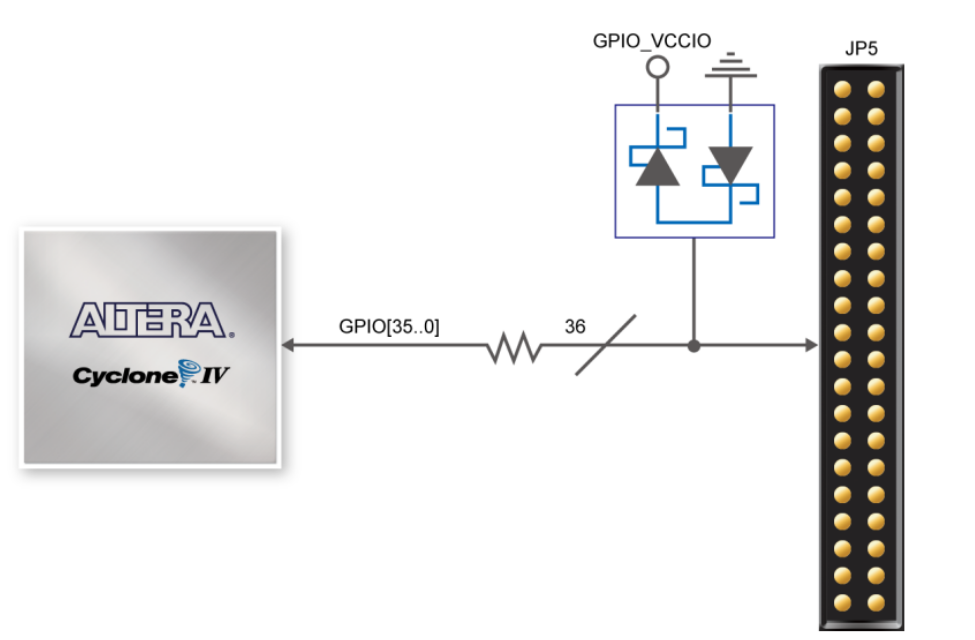
\includegraphics[width= 0.6\textwidth]{figures/pins_fpga_board.png}
                    \caption{\label{fig:pins_fpga_board} Available switches on the development board.}
                \end{center}
            \end{figure}    
        
        \subsection{Switches}
            The DE2i-150 offers 18 switches that can be used during a specific application. But only 8 are going to be available, which are connected to the NEORV32's input pins. The \autoref{tab:sw_i} shows the assignments of the board's switches.
            
            \begin{figure}[!ht]
                \begin{center}
                    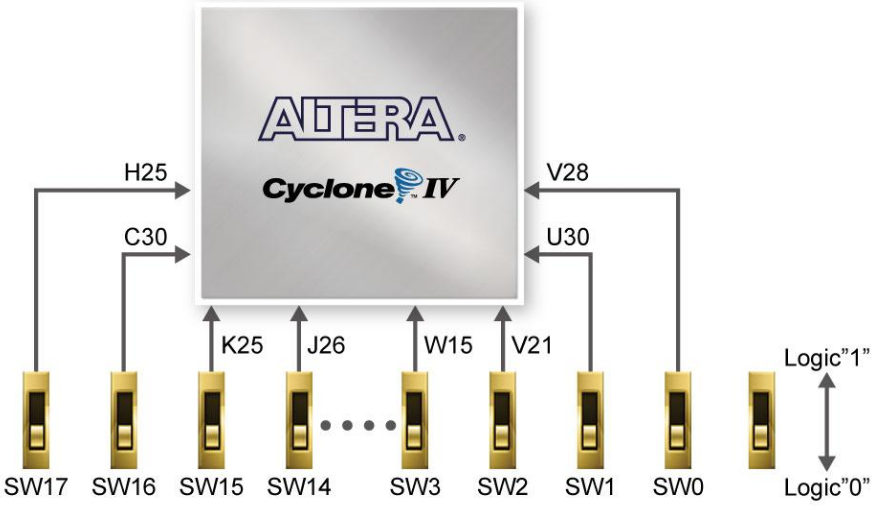
\includegraphics[width= 0.6\textwidth]{figures/sw_fpga_board.png}
                    \caption{\label{fig:sw_fpga_board} Available switches on the development board.}
                \end{center}
            \end{figure}
        
    \section{Interrupt controller}\label{sec:section_p.2}

        To present this peripheral, it is important to define some concepts, such as interruptions, exceptions and traps in a RISC-V architecture. Then, the way in which the microprocessor identifies the interrupt's source, its priority, and the way to handle it needs to be presented, too.
    
        \subsection{Interruptions, exceptions and traps}
    
            First, it is necessary to define interruptions, exceptions and traps. In a RISC-V architecture, interruptions and exceptions will generate a disruption of the on-going execution flow, so that the microprocessor can properly handle a specific event. However, this can occur in two ways: synchronously or asynchronously.
        
            Based on the definitions used in the RISC-V documentation \cite{panesar_2022}, an exception is a synchronous event, as it is a response to some exceptional and unusual condition due to program execution. For instance, some conditions that may raise (cause) an exception include executing a division instruction with a zero divisor, executing an illegal opcode, and a memory protection fault. 
    
    	    Interruption, on the other hand, is an asynchronous event, as it is generated by an external hardware event (which would be external to the microprocessor). These interrupts generally have nothing at all to do with the instructions currently executing; instead, some event, such as pressing a button or a timeout on a timer, informs the microprocessor that a device needs some attention.
    
            Last but not least, in this context, a trap is the transfer of control to a trap handler to determine whether the incoming trap is an interrupt or an exception and call an appropriate handler.
    
    	    When these events occur, the PC register must be saved somewhere, so the microprocessor can resume. Then after handling the event it is possible to load the PC register to continue with the previous execution flow.

        \subsection{Interrupts and exceptions handling}

            To adequately handling the interruptions and exceptions, the NEORV32 has a specific control and status registers (CSRs) for that, which is presented in \autoref{tab:interrupt_csr}. It is composed by 5 CSRs. The most significant bit of mcause will store the interruption's cause (is set to ``1'' if it was generated by an interrupt and ``0'' for an exception). The mip has information regarding the pending interrupts and exceptions waiting to be handled. As presented in \autoref{tab:exception_definitions} and \autoref{tab:interrupt_definitions}\footnotemark, each interrupt and exception have its own priority, so if more than one interrupt happens at the same time, the one with the highest one will be handled first. 

            \footnotetext{\textbf{I-PC}: address of interrupted instruction (instruction has not been executed yet); \textbf{PC}: address of instruction that caused the trap (instruction has been executed); \textbf{ADR}: bad memory access address that caused the trap; \textbf{CMD}: the instruction word that caused the trap (zero-extended if compressed instruction); \textbf{0}: zero.}            

            \begin{table}[!ht]
                \centering
                \caption{Machine trap handling CSRs.}
                \adjustbox{max width=\textwidth}{
                    \begin{tabular}{ccccc}
                        \toprule
                        \textbf{Address} & \textbf{Name [ASM]} & \textbf{Name [C]} & \textbf{ACC} & \textbf{Function} \\
                        \midrule
                        \midrule
                        0x340 & mscratch & CSR\_MSCRATCH & MRW & Machine scratch register \\
                        0x341 & mepc & CSR\_MEPC & MRW & Machine exception program counter \\ 
                        0x342 & mcause & CSR\_MCAUSE & MRW & Machine trap cause \\ 
                        0x343 & mtval & CSR\_MTVAL & MRW & Machine bad address or instruction \\ 
                        0x344 & mip & CSR\_MIP & MRW & Machine interrupt pending register \\ 
                        \bottomrule
                    \end{tabular}
                }
                \label{tab:interrupt_csr}
            \end{table}

            \begin{table}[H]
                \centering
                \caption{Exceptions (synchronous to instruction execution).}
                \adjustbox{max width=\textwidth}{
                    \begin{tabular}{cccccc @{}}
                        \toprule
                        \textbf{Prio.} & \textbf{mcause} & \textbf{ID [C]} & \textbf{Cause} & \textbf{mepc} & \textbf{mtval} \\ 
                        \midrule
                        \midrule
                        1 & 0x00000000 & TRAP\_CODE\_I\_MISALIGNED & instruction address misaligned & I-PC & 0 \\ 
                        2 & 0x00000001 & TRAP\_CODE\_I\_ACCESS & instruction access bus fault & I-PC & 0 \\ 
                        3 & 0x00000002 & TRAP\_CODE\_I\_ILLEGAL & illegal instruction & PC & CMD \\ 
                        4 & 0x0000000B & TRAP\_CODE\_MENV\_CALL & environment call from M-mode & PC & 0 \\ 
                        5 & 0x00000008 & TRAP\_CODE\_UENV\_CALL & environment call from U-mode & PC & 0 \\ 
                        6 & 0x00000003 & TRAP\_CODE\_BREAKPOINT & software breakpoint / trigger firing & PC & PC \\ 
                        7 & 0x00000006 & TRAP\_CODE\_S\_MISALIGNED & store address misaligned & PC & ADR \\ 
                        8 & 0x00000004 & TRAP\_CODE\_L\_MISALIGNED & load address misaligned & PC & ADR \\ 
                        9 & 0x00000007 & TRAP\_CODE\_S\_ACCESS & store access bus fault & PC & ADR \\ 
                        10 & 0x00000005 & TRAP\_CODE\_L\_ACCESS & load access bus fault & PC & ADR \\ 
                        \bottomrule
                    \end{tabular}
                }
            \label{tab:exception_definitions}
        \end{table}

        \begin{table}[H]
            \centering
            \caption{Interrupts (asynchronous to instruction execution).}
            \adjustbox{max width=\textwidth}{
                \begin{tabular}{@{} cccccc}
                    \toprule
                    \textbf{Prio.} & \textbf{mcause} & \textbf{ID [C]} & \textbf{Cause} & \textbf{mepc} & \textbf{mtval} \\ 
                    \midrule
                    \midrule
                    11 & 0x80000010 & TRAP\_CODE\_FIRQ\_0 & fast interrupt request channel 0 & I-PC & 0 \\ 
                    12 & 0x80000011 & TRAP\_CODE\_FIRQ\_1 & fast interrupt request channel 1 & I-PC & 0 \\ 
                    13 & 0x80000012 & TRAP\_CODE\_FIRQ\_2 & fast interrupt request channel 2 & I-PC & 0 \\ 
                    14 & 0x80000013 & TRAP\_CODE\_FIRQ\_3 & fast interrupt request channel 3 & I-PC & 0 \\ 
                    15 & 0x80000014 & TRAP\_CODE\_FIRQ\_4 & fast interrupt request channel 4 & I-PC & 0 \\ 
                    16 & 0x80000015 & TRAP\_CODE\_FIRQ\_5 & fast interrupt request channel 5 & I-PC & 0 \\ 
                    17 & 0x80000016 & TRAP\_CODE\_FIRQ\_6 & fast interrupt request channel 6 & I-PC & 0 \\ 
                    18 & 0x80000017 & TRAP\_CODE\_FIRQ\_7 & fast interrupt request channel 7 & I-PC & 0 \\ 
                    19 & 0x80000018 & TRAP\_CODE\_FIRQ\_8 & fast interrupt request channel 8 & I-PC & 0 \\ 
                    20 & 0x80000019 & TRAP\_CODE\_FIRQ\_9 & fast interrupt request channel 9 & I-PC & 0 \\ 
                    21 & 0x8000001a & TRAP\_CODE\_FIRQ\_10 & fast interrupt request channel 10 & I-PC & 0 \\ 
                    22 & 0x8000001b & TRAP\_CODE\_FIRQ\_11 & fast interrupt request channel 11 & I-PC & 0 \\ 
                    23 & 0x8000001c & TRAP\_CODE\_FIRQ\_12 & fast interrupt request channel 12 & I-PC & 0 \\ 
                    24 & 0x8000001d & TRAP\_CODE\_FIRQ\_13 & fast interrupt request channel 13 & I-PC & 0 \\ 
                    25 & 0x8000001e & TRAP\_CODE\_FIRQ\_14 & fast interrupt request channel 14 & I-PC & 0 \\ 
                    26 & 0x8000001f & TRAP\_CODE\_FIRQ\_15 & fast interrupt request channel 15 & I-PC & 0 \\ 
                    27 & 0x8000000B & TRAP\_CODE\_MEI & machine external interrupt (MEI) & I-PC & 0 \\ 
                    28 & 0x80000003 & TRAP\_CODE\_MSI & machine software interrupt (MSI) & I-PC & 0 \\ 
                    29 & 0x80000007 & TRAP\_CODE\_MTI & machine timer interrupt (MTI) & I-PC & 0 \\ 
                    \bottomrule
                \end{tabular}
            }
            \label{tab:interrupt_definitions}
        \end{table}

            \begin{tcolorbox}[colback=blue!5!white,colframe=blue!75!black,title=Extra information]
                The XIRQ provides up to 32 external interrupt channels configured via the XIRQ\_NUM\_CH, a generic presented in \textit{neor32\_top.vhd} file. Each bit in the xirq\_i input signal vector represents one interrupt channel. If less than 32 channels are configured, only the LSB-aligned channels are used while the remaining ones are left unconnected internally. The actual interrupt trigger type is configured before synthesis using the XIRQ\_TRIGGER\_TYPE and XIRQ\_TRIGGER\_POLARITY, two generics presented in the \textit{neor32\_top.vhd}.
            \end{tcolorbox}
    
            The fast interrupt requests (FIRQs) are better presented in \autoref{fig:firqs}. It is possible to understand what kind of interruptions are available in the NEORV32, furthermore, their priority. It is possible to visualize that the external interrupts has their ``sub-priorities'', which are defined by the external interrupt controller (XIRQ). Its memory map is presented in \autoref{tab:firqs}. It works simmilarly to the ``main interrupt controller'', but specifically for the external ones. 

            \begin{figure}[!ht]
                \begin{center}
                    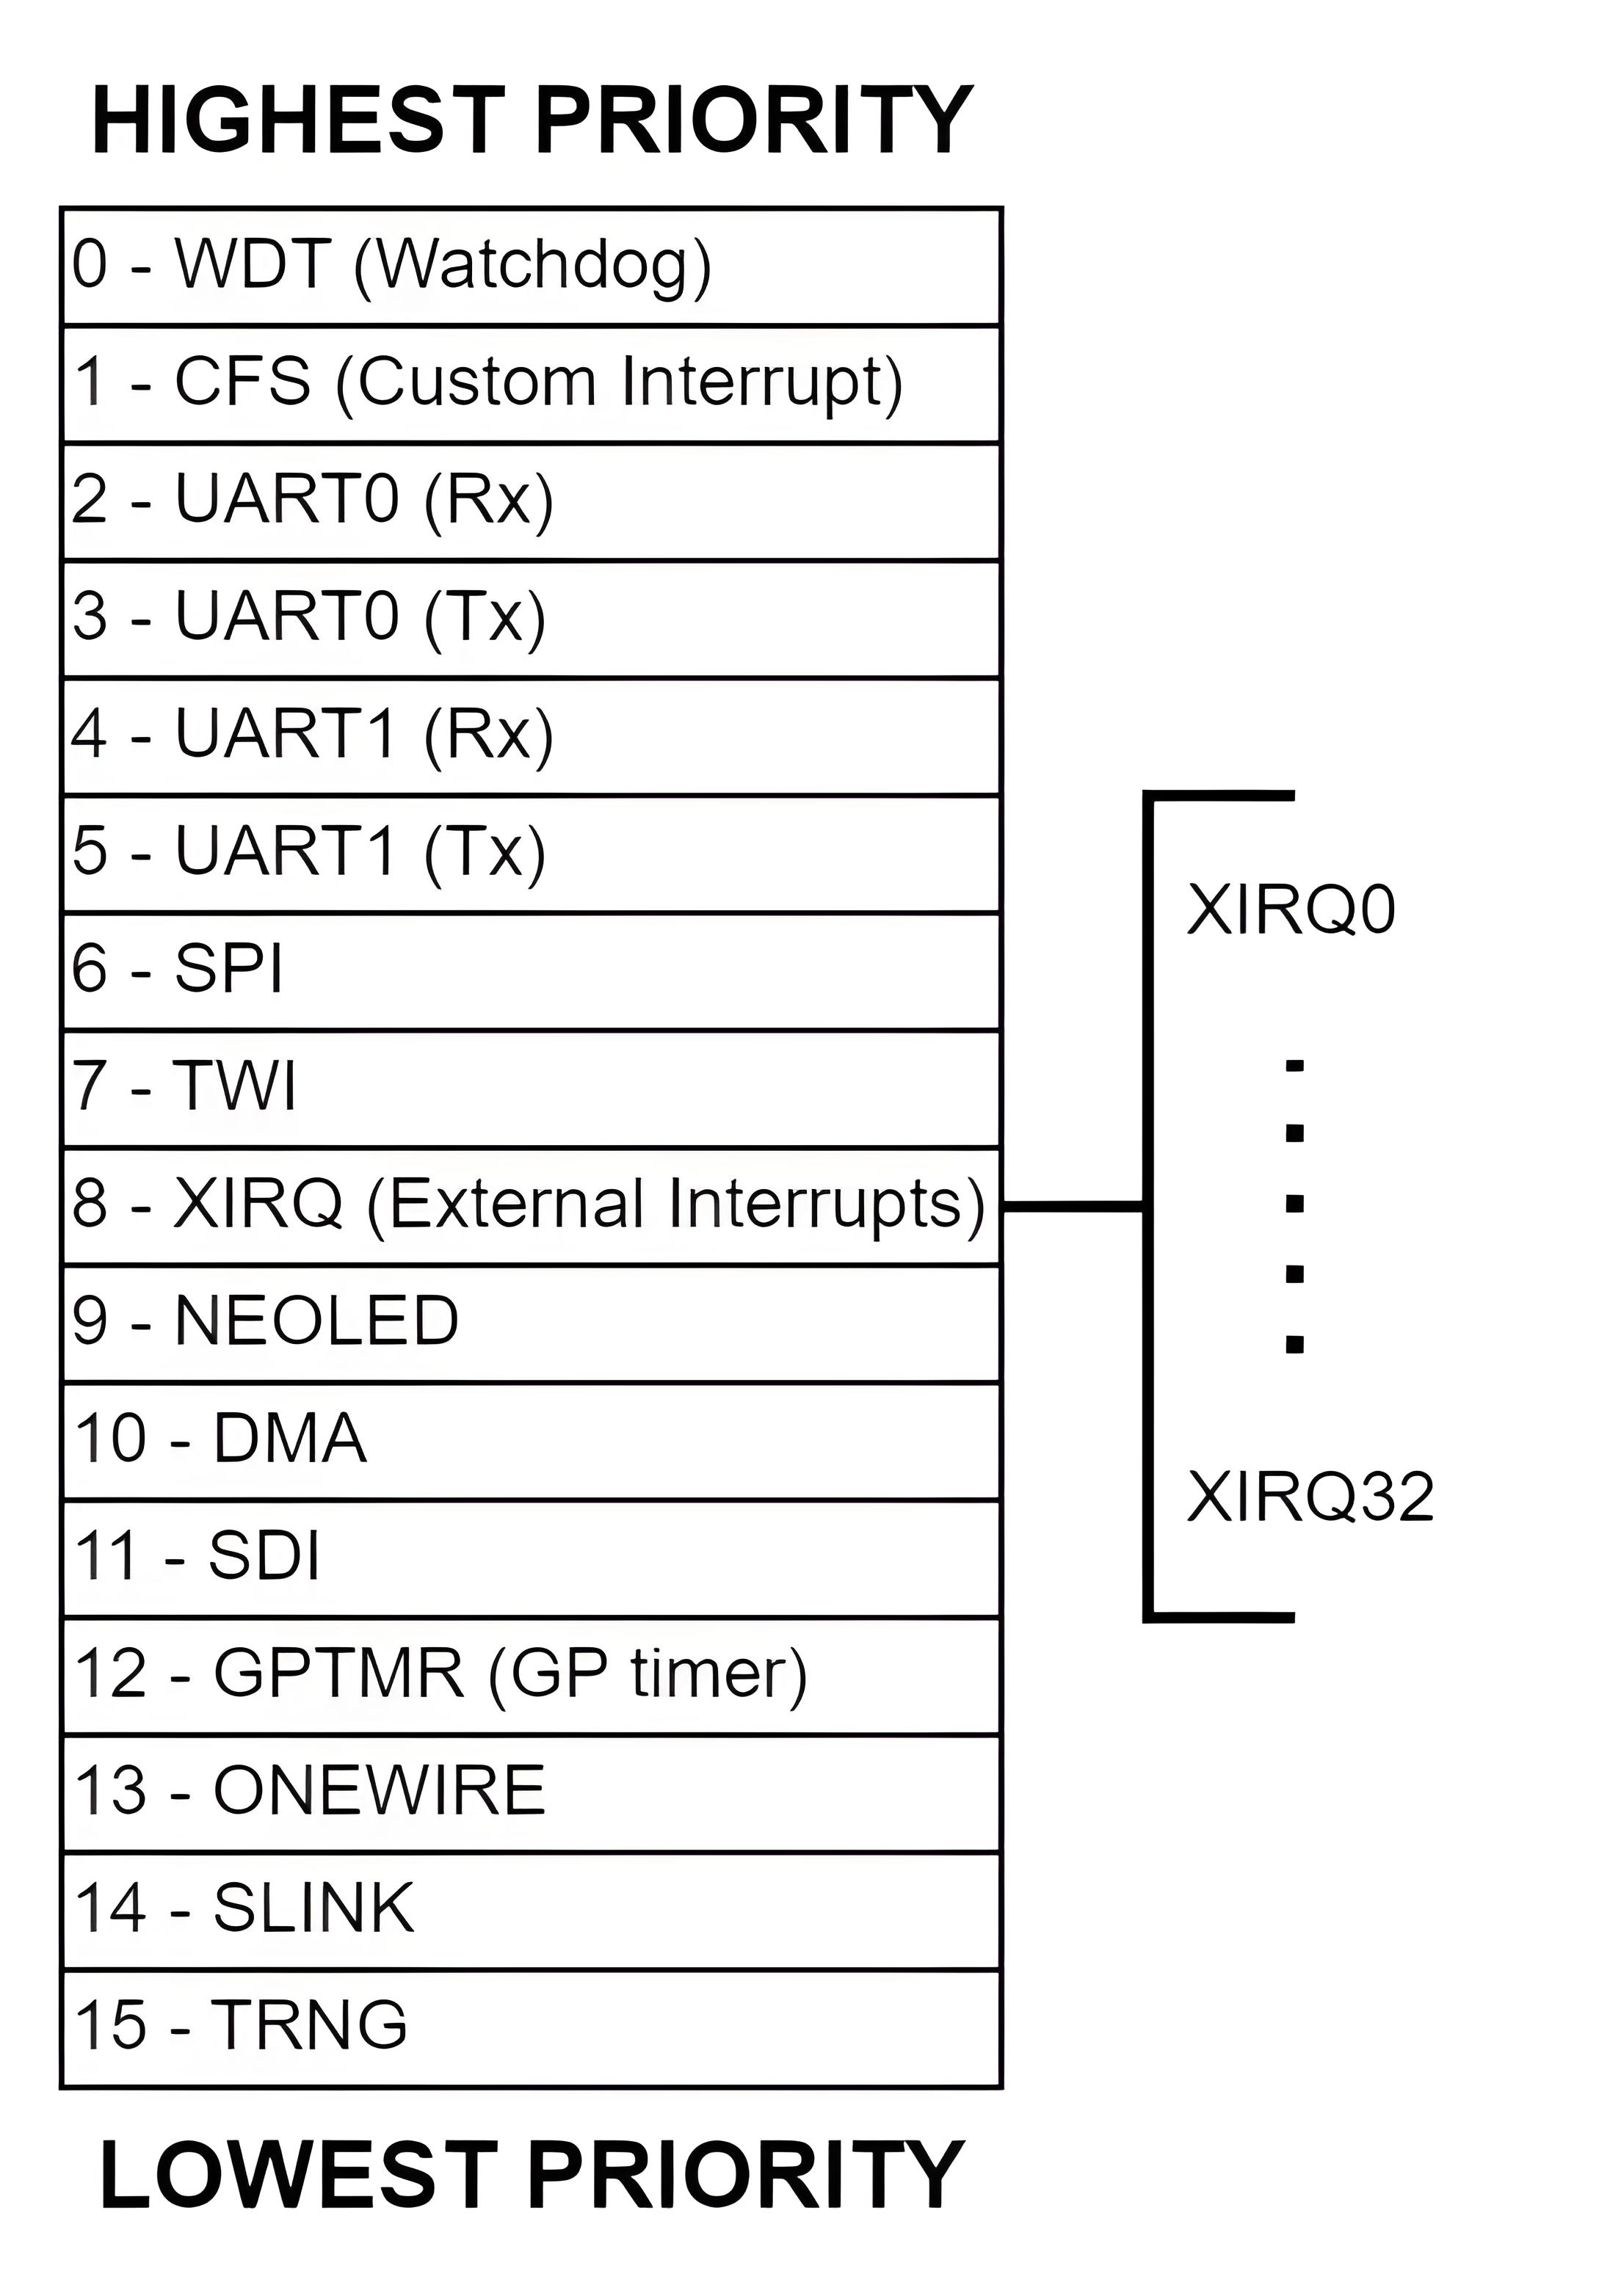
\includegraphics[width= 0.4\textwidth]{figures/firqs.jpeg}
                    \caption{Fast interrupt requests (FIRQs) available.}
                    \label{fig:firqs}
                \end{center}
            \end{figure}

            \begin{table}[!ht]
                \centering
                \caption{XIRQ's memory-mapped registers.}
                \adjustbox{max width=\textwidth}{
                    \begin{tabular}{ccccp{6cm}}
                        \toprule
                        \textbf{Address} & \textbf{Name [C]} & \textbf{Bit(s)} & \textbf{R/W} & \textbf{Description} \\
                        \midrule
                        \midrule
                        0xFFFFFF80 & EIE & 31:0 & r/w & External interrupt enable register (one bit per channel, LSB-aligned) \\
                        0xFFFFFF84 & EIP & 31:0 & r/w & External interrupt pending register (one bit per channel, LSB-aligned); writing 0 to a bit clears the according pending interrupt \\
                        0xFFFFFF88 & ESC & 4:0 & r/w & Interrupt source ID (0..31) of firing IRQ (prioritized!); writing any value will acknowledge the current XIRQ interrupt \\
                        0xFFFFFF8C & - & 31:0 & r/- & Reserved, read as zero \\
                        \bottomrule
                    \end{tabular}
                }
                \label{tab:firqs}
            \end{table}

        \subsection{Input pins and push-buttons}
            The DE2i-150 many ways to interface external devices to generate interruptions. For instance, it has 18 switches that can be used during a specific application, as presented in \autoref{fig:bt_fpga_board}. Only 8 are going to be available, which are connected to the NEORV32's input pins. 

            Furthermore, as presented earlier in \autoref{fig:pins_fpga_board}, it also offer many pins that can be used, too. Here, only two of them are going to be used for generating interruptions.
            
            The \autoref{tab:xirq_i} shows the assignments of the board's switches and pins to be used as interrupt generators.
            
            \begin{figure}[!ht]
                \begin{center}
                    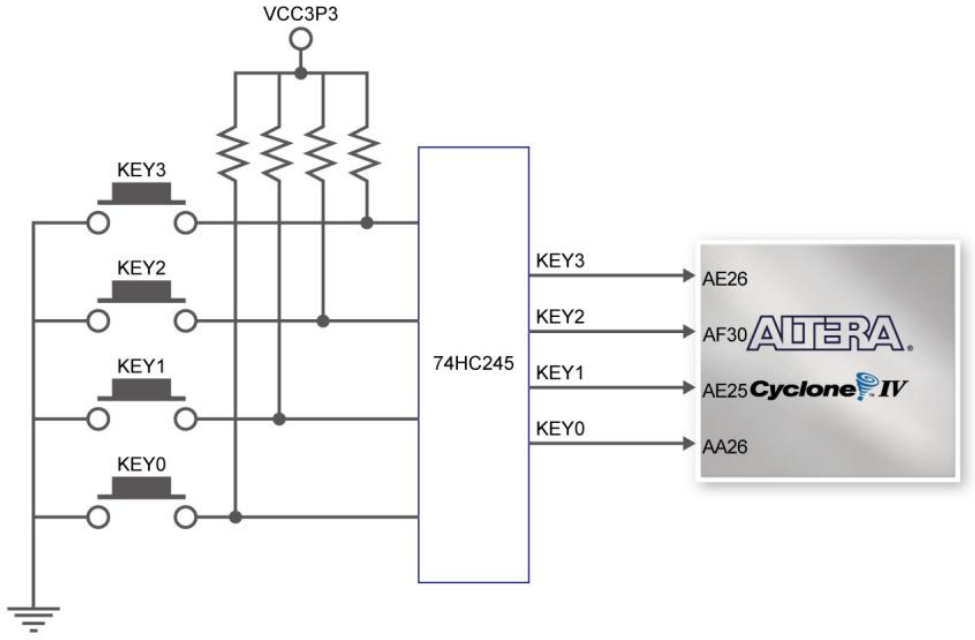
\includegraphics[width= 0.6\textwidth]{figures/bt_fpga_board.png}
                    \caption{\label{fig:bt_fpga_board} Available buttons on the development board.}
                \end{center}
            \end{figure}

    \section{Timers}\label{sec:section_p.3}

        In a microprocessor we can use timers to track time-based events. A timer can be defined as a specialized clock used to measure time intervals. It can function as a stopwatch, counting up from zero or counting down from a set instant. They are often used to generate delays or track the elapsed time. 

        \begin{table}[!ht]
        	\centering
        	\caption{MTIME's memory-mapped registers.}
        	\begin{tabular}{ccccp{4cm}}
        		\toprule
        		\textbf{Address} & \textbf{Name [C]} & \textbf{Bits} & \textbf{R/W} & \textbf{Function} \\
        		\midrule
        		\midrule
        		0xFFFFFF90 & TIME\_LO & 31:0 & r/w & Machine system time, low word \\
        		0xFFFFFF94 & TIME\_HI & 31:0 & r/w & Machine system time, high word \\
        		0xFFFFFF98 & TIMECMP\_LO & 31:0 & r/w & Time compare, low word \\
        		0xFFFFFF9C & TIMECMP\_HI & 31:0 & r/w & Time compare, high word \\
        		\bottomrule
        	\end{tabular}
        	\label{tab:register_map_mtime}
        \end{table}

        In the NEORV32 we have access to the machine system timer (MTIME), which implements a memory-mapped machine timer. It is possible to access the 64-bit system's time via the memory-mapped TIME\_LO and TIME\_HI registers. To configure the timer's interruption, it is necessary to write to other 64-bit registers, which are accessible via the memory-mapped TIMECMP\_LO and TIMECMP\_HI. The interrupt is triggered whenever the content of TIME\_LO and TIME\_HI is greater than or equal to the content of TIMECMP\_LO and TIMECMP\_HI. The interrupt remains active (pending) until TIME\_* becomes less TIMECMP\_* again (either by modifying TIME\_* or TIMECMP\_*). These memories are presented in \autoref{tab:register_map_mtime}, which presents the MTIME's memory map.

        The NEORV32 offers a 32-bit timer, too, the general purpose timer (GPTMR). Its operation is fairly similar to the MTIME. In this peripheral, a 32-bit counter is incremented, which are memory-mapped to COUNT, until reaches the same value stored in the threshold register, the THRES. 

        But in this case it is possible to configure its clock prescaler and its operation mode. For instance, writing to the register GPTMR\_CTRL\_PRSC[2:0], the clock prescaler is configured as presented in \autoref{tab:clock_prescaler}.

        \begin{table}[!ht]
        	\centering
        	\caption{Configuring the clock prescaler}
        	\begin{tabular}{cc}
        		\toprule
        		\textbf{GPTMR\_CTRL\_PRSCx} & \textbf{Resulting clock prescaler} \\
        		\midrule
        		0b000 & 2 \\
        		0b001 & 4 \\
        		0b010 & 8 \\
        		0b011 & 64 \\
        		0b100 & 128 \\
        		0b101 & 1024 \\
        		0b110 & 2048 \\
        		0b111 & 4096 \\
        		\bottomrule
        	\end{tabular}
        	\label{tab:clock_prescaler}
        \end{table}

        Furthermore, it is possible to configure it tu operate in two modes. It is configured trough the GPTMR\_CTRL\_MODE register. If GPTMR\_CTRL\_MODE is equal to ``0'' the timer operates in single-shot mode. So, as soon as COUNT matches THRES an interrupt request is generated and the timer stops its operation (it stops incrementing). However, if GPTMR\_CTRL\_MODE is equal to ``1'' the timer operates in continuous mode. When COUNT matches THRES an interrupt request is generated, but COUNT is automatically reset to all-zero, and then start to increment again. These memories are presented in \autoref{tab:register_map_gptmr}, which presents the GPTMR's memory map.

        \begin{table}[!ht]
        	\centering
        	\caption{GPTMR's memory-mapped registers.}
        	\adjustbox{max width=\textwidth}{
        		\begin{tabular}{ccccp{5cm}}
        			\toprule
        			\textbf{Address} & \textbf{Name [C]} & \textbf{Bit(s), Name [C]} & \textbf{R/W} & \textbf{Function} \\
        			\midrule
        			\midrule
        			0xFFFFFF60 & CTRL & 0 & r/w & Timer enable flag \\
        			& & 3:1 & r/w & 3-bit clock prescaler select \\
        			& & 4 & r/w & Counter mode: 0=single-shot, 1=continuous \\
        			& & 31:5 & r/- & Reserved, read as zero \\
        			0xFFFFFF64 & THRES & 31:0 & r/w & Threshold value register \\
        			0xFFFFFF68 & COUNT & 31:0 & r/w & Counter register \\
        			\bottomrule
        		\end{tabular}
        	}
        	\label{tab:register_map_gptmr}
        \end{table}
                
        
    
    \section{Universal asynchronous receiver-transmitter (UART)}\label{sec:section_p.4}


        Serial communication is very useful when you want to send digital data using few connections. In this type of communication, data is sent sequentially one after the other. There are several serial communication protocols, including SPI, USB, I$^2$C, RS-232, and UART. The use of such protocols became widespread with the use of microcontrollers, such as Arduino.
        
        UART is a serial communication protocol that uses only one wire to transmit (Tx) and another to receive (Rx) the signal, in addition to the reference (GND). The UART communication uses a default configuration between the transmitter and the receiver, which is responsible for defining when the signal starts or ends. It is necessary to define, on both sides, the baud rate, the word size, the start bit, the stop bit, and possibly a parity bit.
        
        Normally, before the beginning of the transmission, the transmitter pin is left at a high state. The start bit is then sent, which consists of a pulse with a low state. After that, the next bits (depending on the size of the previously defined word) are the data bits. The baud rate is used so that it may be possible to detect when the time interval of a bit ends. After sending the word, the signal is placed again at a high state. \autoref{figure:uart} shows the default frame of the UART protocol. Thus, it is possible for the receiver to detect the data sent by the transmitter even without a clock signal of synchronization between both sides.
        
        \begin{figure}[!ht]
            \begin{center}
                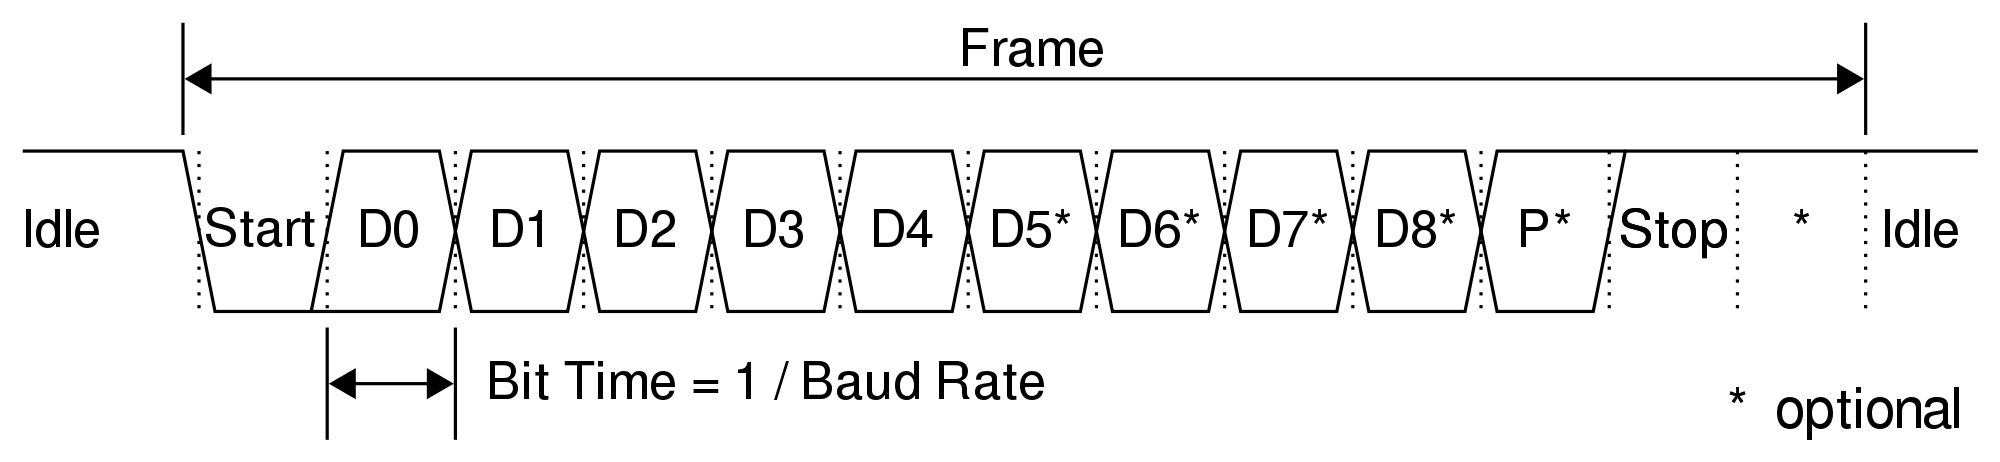
\includegraphics[width= \textwidth]{figures/UART.png}
                \caption{\label{figure:uart} Standard UART Frame}
            \end{center}
        \end{figure}

        In the NEORV32, to use the UART you should configure it, trough the CTRL register. First, you need to enable the UART, setting the UART\_CTRL\_EN. Then, the baud rate is configured, to be able to communicate with another device. The Baud rate is configured via UART\_CTRL\_BAUDx baud[9:0] (baud\_div + 1) and UART\_CTRL\_PRSC[2:0] (clock\_prescaler). Then, the frequency is going to be defined as presented in \autoref{eq:uart}. Furthermore, to read or write data, it is necessary to read or write to the UART\_DATA\_RTX\_*, which is the buffer that stores the Rx and Tx data.

        \begin{equation}
            Baud rate = \frac{fmain}{clock\_prescaler} \cdot \frac{1}{baud\_div + 1}
            \label{eq:uart}
        \end{equation}

        Additionally, it could be mentioned that it is possible to use two channels, UART0 and UART1. Both channels work in the same way. But the priority of channel 0 and 1 are different, as previously shown in \autoref{fig:firqs}.

        \newpage

        \begin{table}[!ht]
        	\centering
        	\caption{UART's memory-mapped registers.}
        	\adjustbox{max width=\textwidth}{
        		\begin{tabular}{ccp{7cm}cp{3cm}}
        			\toprule
        			\textbf{Address} & \textbf{Name [C]} & \textbf{(Bits)Name [C]} & \textbf{R/W} & \textbf{Function} \\
        			\midrule
        			\midrule
        			0xFFFFFFA0 & CTRL & (0)UART\_CTRL\_EN & r/w & UART enable \\
        			& & (1)UART\_CTRL\_SIM\_MODE & r/w & Enable simulation mode \\
        			& & (2)UART\_CTRL\_HWFC\_EN & r/w & Enable RTS/CTS hardware flow-control \\
        			& & (5:3)UART\_CTRL\_PRSC[2:0] & r/w & Baud rate clock prescaler select \\
        			& & (15:6)UART\_CTRL\_BAUD[9:0] & r/w & 12-bit Baud value configuration value \\
        			& & (16)UART\_CTRL\_RX\_NEMPTY & r/- & RX FIFO not empty \\
        			& & (17)UART\_CTRL\_RX\_HALF & r/- & RX FIFO at least half-full \\
        			& & (18)UART\_CTRL\_RX\_FULL & r/- & RX FIFO full \\
        			& & (19)UART\_CTRL\_TX\_EMPTY & r/- & TX FIFO empty \\
        			& & (20)UART\_CTRL\_TX\_NHALF & r/- & TX FIFO not at least half-full \\
        			& & (21)UART\_CTRL\_TX\_FULL & r/- & TX FIFO full \\
        			& & (22)UART\_CTRL\_IRQ\_RX\_NEMPTY & r/w & Fire IRQ if RX FIFO not empty \\
        			& & (23)UART\_CTRL\_IRQ\_RX\_HALF & r/w & Fire IRQ if RX FIFO at least half-full \\
        			& & (24)UART\_CTRL\_IRQ\_RX\_FULL & r/w & Fire IRQ if RX FIFO full \\
        			& & (25)UART\_CTRL\_IRQ\_TX\_EMPTY & r/w & Fire IRQ if TX FIFO empty \\
        			& & (26)UART\_CTRL\_IRQ\_TX\_NHALF & r/w & Fire IRQ if TX not at least half-full \\
        			& & (29:27)ZERO & r/- & Reserved, read as zero \\
        			& & (30)UART\_CTRL\_RX\_OVER & r/- & RX FIFO overflow \\
        			& & (31)UART\_CTRL\_TX\_BUSY & r/- & TX busy or TX FIFO not empty \\
                    \midrule
        			0xFFFFFFA4 & DATA & (7:0)UART\_DATA\_RTX\_* & r/w & Receive/Transmit data \\
        			& & (11:8)UART\_DATA\_RX\_FIFO\_SIZE\_* & r/- & log2(RX FIFO size) \\
        			& & (15:12)UART\_DATA\_TX\_FIFO\_SIZE\_* & r/- & log2(RX FIFO size) \\
        			  & Reserved & (31:16)ZERO & r/- & Reserved, read as zero \\
        			\bottomrule
        		\end{tabular}
        	}
        	\label{tab:uart_registers}
        \end{table}

        \subsection{UART interface}

            To use the UART in the development board, it is used the J6, a RS-232 connector. And a IC makes the conversion of RS-232 to UART, as presented in \autoref{fig:uart_development_board}.  
            
            \begin{figure}[!ht]
                \begin{center}
                    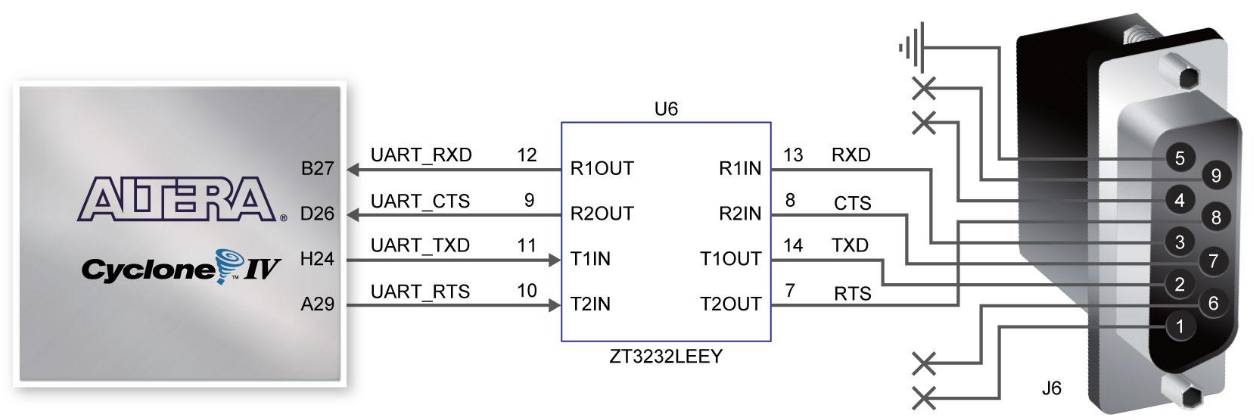
\includegraphics[width= 0.6\textwidth]{figures/uart_development_board.png}
                    \caption{\label{fig:uart_development_board} UART interface in the development board.}
                \end{center}
            \end{figure}